\documentclass[12pt,a4paper]{memoire-umons}

\usepackage[utf8]{inputenc}
\usepackage[T1]{fontenc}
\usepackage[francais]{babel}
\usepackage{amssymb,amsmath,amsthm}
\usepackage{hyperref}% hyperliens dans le PDF, pas pour impression

%------Notes------------
\newcounter{note}[section]
\newenvironment{note}[1][]
{	
	
	\refstepcounter{note}
	\noindent
	\underline{\textbf{Remarque \arabic{section}.\arabic{note}:}}
	
	
	\begin{center}
		\begin{em}
		}
		{
		\end{em}	
	\end{center}

}
%----------------------
\usepackage{xcolor}
\usepackage{tikz}


\graphicspath{{./figures/}}

\title{Générateur Dynamique de Contenu Static}
\author{Maxime \textsc{De Wolf}}
\date{2017--2018}
\directeur{Decan Alexandre}
\service{Sciences Informatiques}
\rapporteurs{}
\discipline{informatiques}


%%%%%%%%%%%%%%%%%%%%%%%%%%%%%%%%%%%%%%%%%%%%%%%%%%%%%%%%%%%%%%%%%%%%%%%%
%% Vos macros


%%%%%%%%%%%%%%%%%%%%%%%%%%%%%%%%%%%%%%%%%%%%%%%%%%%%%%%%%%%%%%%%%%%%%%%%

% Compile uniquement certains morceaux sans perdre les références
% automatiques et la table des matières des parties déjà compilées :
%\includeonly{introduction,chapitre1}

\begin{document}
% Éventuellement utiliser l'environnement « preface » pour avoir une
% numérotation des pages en chiffres romains.
\tableofcontents

\chapter{Introduction}

	
\section{Cahier des charges}

	Cette section a pour rôle de présenter le cahier des charges de ce projet. Nous introduirons également le concept de générateur de contenu static. La seconde partie de cette section listera quelques cas d'utilisation afin d'illustrer le fonctionnement souhaité par ce projet. Notez que les fonctionnalités en elles-même seront détaillées dans la Section 4.\\
	
	Le cahier des charges de ce projet est volontairement resté assez flou. En effet, les seules consignes données étaient de concevoir un générateur de contenu static qui donnait à l'utilisateur une grande souplesse d'utilisation. La simplicité d'utilisation du générateur est également un critère important. Afin de clarifier ce que veut dire "souplesse d'utilisation", quelques cas d'utilisations seront illustrer dans cette section.\\
	
	
	\subsection{Générateur de contenu static}
	
		Un générateur de contenu static sert -comme son nom l'indique- à générer du contenu. Il sera qualifié de "static" si ce contenu ainsi généré est prêt à l'emploi et ne nécessite plus de transformation afin d'être utile. A savoir que les générateurs de contenu static sont très utilisés pour produire des sites web statics. Celui-ci aura une vocation un peu plus générale car il permettra de générer à peu près n'importe quel type de contenu static. Leur utilisation est souvent lié au concept de \textit{templates} qui permettent de séparer les informations de la mise en page en elle-même. La Figure \ref{fig:use_of_generator} montre une utilisation type de ce genre de générateur.\\
		
		\begin{figure}
			\begin{center}
				\begin{tikzpicture}
				\coordinate (Data) at (-3, 0);
				\coordinate (Template) at (-1, 1);
				\coordinate (Content) at (2, 0);
				\coordinate (Center) at (-1, 0);
				
				\draw (-4, 0) circle (1) ;
				\draw (-4, 0) node{$\text{Données}$};
				\draw[>=latex, ->] (Data) -- (Center);
				
				\draw[rounded corners]  (2, -1) rectangle(4, 1);
				\draw (3, 0) node{$\text{Contenu}$};
				\draw[>=latex, ->] (Center) --(Content);
				
				\draw(-2, 1) rectangle(0, 3);
				\draw (-1, 2) node{$\text{Template}$};
				\draw[>=latex, ->]  (Template) -- (Center);
			\end{tikzpicture}
			\caption{Utilisation type d'un générateur de contenu static}
			\label{fig:use_of_generator}
			\end{center}
		\end{figure}

	\subsection{Cas d'utilisations}
	
		Nous distinguons principalement trois cas d'utilisations propres aux générateurs de contenu statique. Chacun d'entre eux sera illustré à l'aide d'une figure. Nous appellerons ces trois cas comme suit: \textit{OneToAll}, \textit{AllToOne} et \textit{AllToMany}.\\
		
		\subsubsection*{OneToAll}
		
			La cas \textit{OneToAll} désigne l'utilisation d'un générateur de contenu static afin de générer plusieurs fichiers en sorties à partir d'un seul fichier en entré. Cela correspond, par exemple, à afficher un produit par page à partir d'un fichier contenant l'ensemble des produits disponibles. Cela se traduit par la Figure \ref{fig:OneToAll} en considérant que \textbf{n} est le nombre de produits contenus dans le fichier.
			
			\begin{figure}
				\begin{center}
					\begin{tikzpicture}
					\coordinate (Data) at (-3, 0);
					\coordinate (Template) at (-1, 1);
					\coordinate (Content) at (2, 0);
					\coordinate (Center) at (-1, 0);
					
					\draw (-4, 0) circle (1) ;
					\draw (-4, 0) node{$\text{Données}$};
					\draw[>=latex, ->] (Data) -- (Center) node[near start, above] {$1$};
					
					\draw[rounded corners]  (2, -1) rectangle(4, 1);
					\draw (3, 0) node{$\text{Contenu}$};
					\draw[>=latex, ->] (Center) --(Content) node[near end, above] {$n$};
					
					\draw(-2, 1) rectangle(0, 3);
					\draw (-1, 2) node{$\text{Template}$};
					\draw[>=latex, ->]  (Template) -- (Center) node[midway, right]{1};
					\end{tikzpicture}
					\caption{Représentation du cas \textbf{OneToAll}.}
					\label{fig:OneToAll}
				\end{center}
			\end{figure}
		
		\subsubsection*{AllToOne}
		
			Le second cas, \textit{AllToOne}, est le cas inverse de \textit{OneToAll}. En effet, ce cas désigne l'utilisation d'un générateur de contenu static pour générer un seul fichier à partir de plusieurs. En pratique, cela consiste par exemple à afficher l'intégralité des posts d'un blog sur une seule page, chaque page étant symbolisée par un fichier. Cela donne la Figure \ref{fig:AllToOne} où \textbf{n} est le nombre de fichiers contenant un post.
		
			\begin{figure}
				\begin{center}
					\begin{tikzpicture}
					\coordinate (Data) at (-3, 0);
					\coordinate (Template) at (-1, 1);
					\coordinate (Content) at (2, 0);
					\coordinate (Center) at (-1, 0);
					
					\draw (-4, 0) circle (1) ;
					\draw (-4, 0) node{$\text{Données}$};
					\draw[>=latex, ->] (Data) -- (Center) node[near start, above] {$n$};
					
					\draw[rounded corners]  (2, -1) rectangle(4, 1);
					\draw (3, 0) node{$\text{Contenu}$};
					\draw[>=latex, ->] (Center) --(Content) node[near end, above] {$1$};
					
					\draw(-2, 1) rectangle(0, 3);
					\draw (-1, 2) node{$\text{Template}$};
					\draw[>=latex, ->]  (Template) -- (Center) node[midway, right]{1};
					\end{tikzpicture}
					\caption{Représentation du cas \textbf{AllToOne}.}
					\label{fig:AllToOne}
				\end{center}
			\end{figure}
			
		\subsubsection*{AllToMany}
			
			Le dernier cas est celui que nous appellerons \textit{AllToMany}. Ce cas est en fait une généralisation des deux cas précédant. Effectivement, \textit{AllToMany} désigne l'utilisation d'un générateur de contenu static afin de générer plusieurs fichiers en sortis à partir de plusieurs fichier d'entrés. Mis en contexte, il désigne par exemple la génération de fichiers contenant chacun plusieurs posts à partir de fichiers contenant chacun un post. La Figure \ref{fig:AllToMany} permet une vision plus claire de ce cas où \textbf{n} désigne le nombre de fichier contenant chacun un post et \textbf{m} le nombre de pages (resp. fichiers) contenant un certains nombre de posts.\\
			
			\begin{figure}
				\begin{center}
					\begin{tikzpicture}
					\coordinate (Data) at (-3, 0);
					\coordinate (Template) at (-1, 1);
					\coordinate (Content) at (2, 0);
					\coordinate (Center) at (-1, 0);
					
					\draw (-4, 0) circle (1) ;
					\draw (-4, 0) node{$\text{Données}$};
					\draw[>=latex, ->] (Data) -- (Center) node[near start, above] {$n$};
					
					\draw[rounded corners]  (2, -1) rectangle(4, 1);
					\draw (3, 0) node{$\text{Contenu}$};
					\draw[>=latex, ->] (Center) --(Content) node[near end, above] {$m$};
					
					\draw(-2, 1) rectangle(0, 3);
					\draw (-1, 2) node{$\text{Template}$};
					\draw[>=latex, ->]  (Template) -- (Center) node[midway, right]{$1$};
					\end{tikzpicture}
					\caption{Représentation du cas \textbf{AllToMany}.}
					\label{fig:AllToMany}
				\end{center}
			\end{figure}
		
		\subsection{Cas non-couverts}
			Un lecteur attentif aura remarqué que nous ne discutons pas de la multiplicité au niveau de l'application des \textit{templates}. Pour un soucis de complétude, nous les listerons dans cette section. Ils feront éventuellement parti de l'implémentation finale si le temps nous le permet. Nous appellerons ces cas \textit{MultiTemplatesIn} et \textit{MultiTemplatesOut}.
			
			 Notez que ces cas d'utilisations seraient réalisables sans implémentation additionnelle. Malheureusement cela impliquerait quelques contraintes pour l'utilisateur ce qui nuirait à la souplesse d'utilisation de notre générateur de contenu static. Nous discuterons de cela plus avant dans la Section 5.
			
			\subsubsection*{MultiTemplatesIn}
				Ce cas d'utilisation implique  d'utiliser un générateur de contenu static dans le but de produire un fichier contenant plusieurs fois les mêmes données mais chaque fois agencées par un \textit{template} différent. Nous n'avons pas trouvé d'exemple pratique mais cela pourrait servir à comparer plusieurs \textit{templates} entre eux. La Figure \ref{fig:MultiTemplatesIn} illustre ce cas plus clairement, où \textbf{n} est le nombre de \textit{templates} à appliquer sur le fichier de données.
				
				\begin{figure}
					\begin{center}
						\begin{tikzpicture}
						\coordinate (Data) at (-3, 0);
						\coordinate (Template) at (-1, 1);
						\coordinate (Content) at (2, 0);
						\coordinate (Center) at (-1, 0);
						
						\draw (-4, 0) circle (1) ;
						\draw (-4, 0) node{$\text{Données}$};
						\draw[>=latex, ->] (Data) -- (Center) node[near start, above] {$1$};
						
						\draw[rounded corners]  (2, -1) rectangle(4, 1);
						\draw (3, 0) node{$\text{Contenu}$};
						\draw[>=latex, ->] (Center) --(Content) node[near end, above] {$1$};
						
						\draw(-2, 1) rectangle(0, 3);
						\draw (-1, 2) node{$\text{Template}$};
						\draw[>=latex, ->]  (Template) -- (Center) node[midway, right]{$n$};
						\end{tikzpicture}
						\caption{Représentation du cas \textbf{MultiTemplatesIn}.}
						\label{fig:MultiTemplatesIn}
					\end{center}
				\end{figure}
				
			
			\subsubsection*{MultiTemplatesOut}
				Ce cas d'utilisation est similaire au précédent, il implique également l'application de plusieurs \textit{templates} sur un même fichier de données. La différence vient du fait que \textit{MultiTemplatesOut} produit un fichier en sortie par \textit{template} appliqué. En pratique, cela veut par exemple dire que pour un fichier contenant les informations propres à un \textit{CV} on veuille générer un fichier \LaTeX et une page web. Ces deux contenus contiendraient les mêmes informations mais l'un pourra être imprimé (une fois le PDF produit) et l'autre sera mis à disposition sur Internet. Cela se traduit par la Figure \ref{fig:MultiTemplatesOut} où \textbf{n} est le nombre de \textit{templates} à appliquer sur le fichier.
				
				\begin{figure}
					\begin{center}
						\begin{tikzpicture}
						\coordinate (Data) at (-3, 0);
						\coordinate (Template) at (-1, 1);
						\coordinate (Content) at (2, 0);
						\coordinate (Center) at (-1, 0);
						
						\draw (-4, 0) circle (1) ;
						\draw (-4, 0) node{$\text{Données}$};
						\draw[>=latex, ->] (Data) -- (Center) node[near start, above] {$1$};
						
						\draw[rounded corners]  (2, -1) rectangle(4, 1);
						\draw (3, 0) node{$\text{Contenu}$};
						\draw[>=latex, ->] (Center) --(Content) node[near end, above] {$n$};
						
						\draw(-2, 1) rectangle(0, 3);
						\draw (-1, 2) node{$\text{Template}$};
						\draw[>=latex, ->]  (Template) -- (Center) node[midway, right]{$n$};
						\end{tikzpicture}
						\caption{Représentation du cas \textbf{MultiTemplatesOut}.}
						\label{fig:MultiTemplatesOut}
					\end{center}
				\end{figure}
				
	
\section{Etat de l'art}
	%todo justifier le choix des référence
	Cette section détaille, de manière non-exhaustive, l'existence d'autres générateurs de contenu statique similaires à ce projet. Leurs fonctionnalités principales seront présentées afin d'être comparées avec notre propre générateur.\\
	
	Ces générateurs de contenu statique ont été choisis grâce à StaticGen \cite{StaticGen} qui établie un classement d'un grand nombre de ces générateurs sur base de leur popularité sur GitHub. Parmi tous ceux qui y sont listés, nous en avons choisis trois comme étalons pour notre projet. Il s'agit de Jekyll, Pellican et Lektor.\\
	
	Nous pouvons expliquer ces choix comme suit: Jekyll est le générateur \textit{open-source} le plus populaire. Il s'agit donc d'un bon point de comparaison. Ensuite, Pellican est le générateur le plus populaire écrit en Python. Comme notre projet est également réalisé en Python, nous trouvons qu'il s'agit également d'une comparaison intéressante. Enfin, Lektor est le quatrième générateur le plus populaire réalisé en Python. Il offre cependant une plus grande souplesse d'utilisation que Pellican. Comme la souplesse d'utilisation est un critère important pour notre projet, nous avons jugé bon de l'ajouter à notre comparaison.
	
	\subsection*{Pelican}
	Pelican \cite{Pelican} est un générateur de site web statique dont les principales fonctionnalités sont:
	\begin{itemize}
		\item Le support de \textit{pages} (e.g. "Contact", ...)
		\item Le support d'\textit{articles} (e.g. posts d'un blog)
		\item La régénération rapide de fichiers grâce à un système de caches et d'écriture sélective.
		\item La gestion de thèmes créés à partir de \textit{templates Jinja2}
		\item La publication d'articles dans plusieurs langues
	\end{itemize}
	
	\subsection*{Lektor}
	Lektor \cite{Lektor} est également un générateur de site web statique. Ses principales fonctionnalités sont les suivantes:
	
	\begin{itemize}
		\item Un système de construction intelligent qui ne reconstruit que le \\contenu qui a été modifié
		\item Un outil graphique qui permet la modification de pages sans toucher au code source
		\item Utilisation de système de \textit{templates Jinja2} pour le rendu du contenu
		\item Un outil permettant la création relativement simple de sites web multilingues
	\end{itemize}
	
	On peut donc en conclure que c'est un outil assez similaire à Pelican sauf que Lektor propose un outil graphique pour l'édition de contenu.
	
	\subsection*{Jekyll}
	Enfin, Jekyll \cite{Jekyll} est le plus connu des générateurs de sites web statiques \textit{open source}. Il est écrit en \textit{Ruby} à la différence de Pelican et Lektor, écrits en \textit{Python}. Voici ses principales fonctionnalités:
	
	\begin{itemize}
		\item Utilisation de \textit{templates Liquid}
		\item Support de contenu de type \textit{pages} (e.g "Contact", "Accueil", ...) et \textit{articles} (e.g. posts d'un blog)
		\item Lancement d'un serveur local pour observer le rendu graphique des fichiers générés\\
	\end{itemize}
	
	%todo conclure l'état de l'art
	Malgré leurs différences, chacun de ces générateurs de sites web statiques fonctionnent selon le cas d'utilisation \textit{AllToOne} (voir Figure \ref{fig:ManyToOne}). Ce cas est très utilisé dans le cas de sites web de type blog d'où sa popularité.
\section{Analyse fonctionnelle}

	Cette section est destinée à justifier les choix de conception de ce projet afin de remplir le cahier des charges. Certains choix seront inspirés directement de solutions existantes listées dans la section précédente.
	
	La section suivante, sera directement liée à celle-ci car elle expliquera comment ces choix seront techniquement mis en œuvre lors de la phase d'implémentation.
	
	\subsection{Abstraction des données}
		Un des points forts de notre générateur de contenu statique est de pouvoir abstraire les données qu'il traite. Grâce à ce mécanisme, l'utilisateur est capable de manipuler une grande diversité de type de donnée sans avoir à adapter ses manipulations. Dit autrement, cela permet à l'utilisateur de travailler de la même manière avec plusieurs types de données différents sans avoir à adapter ses requêtes. Cela donne également la possibilité de manipuler ensemble des données  syntaxiquement différentes mais sémantiquement les mêmes. Dans ce cas, pour parler des données traitées, nous utiliserons le mot "\textbf{item}" introduit dans la section 2.1.
		
	\subsection{Configuration}
	%todo a qui profite la prog. modulaire ?
		Un autre point fort de notre générateur de contenu statique est qu'il est facilement configurable. En effet, il est possible de configurer son répertoire de travail ainsi que le moteur de rendu utilisé pour les \textit{templates}. Mais cela reste une fonctionnalité assez classique. L'originalité de notre système de configuration vient du fait qu'il est également possible d'y ajouter des modules \textit{Python 3} en plus des modules de bases que nous proposons. Cela permet à l'utilisateur d'y ajouter des fonctionnalités qu'il aurait lui-même développé pour que notre générateur réponde au mieux à ses besoins.
		

	\subsection{Règles de génération}
	%todo expliquer le principe général des règles 
		Pour ce qui est de l'utilisation en elle-même de notre générateur de contenu statique, nous avons pensé à un système de règles relativement intuitif.
		Ces règles sont divisées en plusieurs parties appelées \textbf{champs}. Chaque champs (ou ensemble de champs) représente un paramètre du générateur de contenu statique.	L'explication du fonctionnement de ces règles est approfondies dans la section suivantes. Ces règles permettent également à l'utilisateur de créer des variables qu'il peut ensuite utilisées dans le \textit{template}. Ces règles sont contenues dans un fichier qui sera passé en paramètre à notre programme qui les exécutera une par une. Chacune de ces règles symbolisera un des trois cas d'utilisation exposé en Section 2: \textit{AllToOne, OneToAll} et \textit{AlltoMany}.
		
	\subsection{Transformation des données}
	
		Une fonctionnalité importante de notre générateur de contenu statique est la possibilité d'appliquer des transformations aux données en cours de traitement. Cela peut par exemple permettre à l'utilisateur de formater certaines données avant de les injecter dans le \textit{template}. Afin de faciliter ce processus pour l'utilisateur, nous mettons aussi à sa disposition des méta-fonctions. Ces fonctions sont au nombre de trois: \textbf{map}, \textbf{reduce}, \textbf{filter}. 
		
		\textit{Map} est une méta-fonction qui permet d'appliquer une fonction à chaque \textit{item} d'un ensemble d'\textit{items}. Le résultat est donc un nouvel ensemble d'\textit{items} dont chaque  \textit{item} est le résultat de l'application de la fonction sur un \textit{item} de l'ensemble initial.
		
		\textit{Reduce} est une méta-fonction qui applique une fonction sur un ensemble d'\textit{items} deux par deux. L'un des deux items passé à cette fonction est le résultat obtenu à partir de la paire d'\textit{items} précédente. Le résultat est donc accumulé jusqu'à ce que la fonction ait été appliquée sur tout les \textit{items}. Le résultat de cette méta-onction est donc un unique \textit{item}.
		
		\textit{Filter} est une méta-fonction qui applique une fonction booléenne à chaque membre d'un ensemble d'\textit{item}. Le résultat de cette méta-fonction est un nouvel ensemble d'\textit{items} contenant uniquement les \textit{items} dont le résultat de la fonction est \texttt{True}.
		
		Ces trois méta-fonctions permettent à l'utilisateur de transformer les données en cours de traitement avec une très grande flexibilité.\\
		
		En plus de ces méta-fonctions, nous mettons également à disposition de l'utilisateur toute une série de fonctions de base pour l'aider à traiter au mieux ses données.
	
	\subsection{Ajout de méta-données}
	
		Chaque donnée traitée par notre générateur de contenu statique se voit assigner des méta-données en fonction des différentes transformations que celle-ci subit. Ces méta-données peuvent donc par exemple représenter le nom du fichier duquel les données ont été chargées, l'extension du fichier, ... Ces méta-données sont ensuite utilisable dans le \textit{template} au même titre que les données elles-mêmes.
		
	\subsection*{Syntaxe}
	
		Un objectif important de notre générateur de contenu statique est de fournir à l'utilisateur une syntaxe compacte et intuitive. Cela s'applique tout particulièrement aux règles de générations qui est la partie la plus complexe à gérer pour un utilisateur.\\
		
		D'une part nous n'obligeons l'utilisateur qu'à manipuler des fichiers au format relativement simple, à savoir au format \textit{YAML}. D'autre part, les expressions utilisée dans les règles de générations constituent une grande partie de cette complexité.
		
		Nous avons donc choisi de faire en sorte que le résultat d'une fonction soit automatiquement passée en paramètre à la fonction suivante grâce à l'opérateur ">>". Cela permet ainsi de bien séparer chaque appel de fonction au niveau syntaxique. Et donc cela améliore aussi la lisibilité.
		
		De plus, ce comportement est assez intuitif car appliquer des fonctions une à une sur des données dans le but de les "raffiner" est typiquement ce que l'utilisateur souhaite faire. 
	
	\subsection{Système de fichiers \textit{logs}}
	
		\begin{note}
			Cette fonctionnalité n'est pas présente dans notre générateur de contenu statique car elle n'était pas spécifiée dans le cahier des charges. Néanmoins, nous trouvons que celle-ci est intéressante, c'est pourquoi nous la détaillons quand même dans cette sous-section.
		\end{note}
	
		Un système de fichiers \textit{logs} permettrait de faciliter la correction des règles lorsque les fichiers en sorties ne correspondent pas à ce que l'utilisateur attend. Ces fichiers \textit{logs} n'ont comme utilité que de lister l'historique des fonctions appliquées pas à pas pour chaque champ de chaque règle. L'utilisateur n'a donc plus qu'à repérer quelle règle et quel champ n'agit pas comme il le voudrait.\\
		
		Ce système viserait à atteindre l'objectif de simplicité d'utilisation -et d'aide à l'utilisation dans ce cas-ci- mentionné dans le cahier des charges en Section 2.
		
		
\section{Analyse technique}
	Cette section est destinée à détailler les techniques mises en œuvres afin d'implémenter les différentes fonctionnalités décrites dans la section précédente. Le but de cette analyse technique est de montrer le raisonnement qui a conduit à la structure actuelle de notre générateur de contenu statique. Nous n'exposerons donc pas les détails d'implémentations. Si cela vous intéresse, le code source à disposition sur \url{https://github.com/MaximeDeWolf/DGSC/tree/master/code/src}.
	
	\subsection{Règles}
	%todo trouver un autre nom pour "target" qui suggère une entrée
	%todo mieux expliquer ce que désigne les champs d'une règle + exemple
	
	Une règle de génération est le moyen que nous mettons à disposition à l' utilisateur pour que celui-ci spécifie à notre générateur de contenu statique pour désigner le comportement que celui-ci doit adopter.
	Typiquement, une règle représente un cas d'utilisation. Il s'agit donc d'un des points les plus importants du projet. Cette sous-section explique donc en détail les différents éléments qui définissent ces règles ainsi que leur structure.
	
	\subsubsection*{Le format}
	
		Le format des fichiers de règles se doit de posséder deux qualités importantes. La première est d'être facilement compréhensible par l'utilisateur aussi bien lors de la lecture que de l'écriture. La deuxième est de pouvoir être analysé facilement par notre générateur de contenu statique dans le but d'y lire les informations nécessaire à son fonctionnement.
		
		Nous avons donc choisis le format \textit{YAML} pour stocker ces règles. Chaque fichier de règles contient donc une liste de règles. Ces règles contiennent chacune quatre champs qui eux-mêmes contiennent une expression. Ce sont ces expressions qui seront évaluées par notre générateur. La Figure \ref{fig:rule:format} illustre le format type d'un fichier de règles.
		
		\begin{figure}[!]
			\centering
			\lstinputlisting[inputencoding=utf8/latin1]{codeSample/ruleFormat.yaml}
			\caption{Format d'un fichier de règles de notre générateur}
			\label{fig:rule:format}
		\end{figure}
		
	\subsubsection*{Les expressions}
	
	\subsubsection*{Les champs}
		Ces règles possèdent quatre champs obligatoires: \textit{target}, \textit{template}, \textit{data} et \textit{output}. Comme expliqué dans la précédente section, chacun de ces champs (ou ensemble de champs) permet de  contrôler les paramètres de notre générateur. \textit{target} et \textit{output} représentent le contenudu générateur tandis que \textit{template} et \textit{data} représentent respectivement le \textit{template} et les données. Les particularités et fonctions de chacun de ces champs sont expliqués ci-dessous.
		
		
		\subsubsection*{Target}
			Le champ \textit{target} contient une expression destinée à être lue par notre générateur. Le résultat de cette expression sert à définir la multiplicité du paramètre "contenu" de la règle. Cela définit le nombre de fois que les autres champs de la règles courantes doivent être évalués. A chaque itération de ce processus un \textit{item} différent est stocké dans une variable appelée \textit{current}. Cette variable est ensuite utilisable dans les autres champs de la règle courante.
		
		\subsubsection*{Template}
		%todo clarifier quel moteur de template gère le cas MultiTemplatesIn
			Ce champs contient une expression destinée à être évaluée par notre générateur de contenu statique. Le résultat de cette expression à désigner le \textit{template} à utiliser sur les données chargées grâce au champ \textit{data}.\\
			
			La multiplicité de ce paramètre est volontairement bloquée à un. En effet, cela simplifie ainsi l'utilisation de notre générateur de contenu statique bien cela limite également souplesse d'utilisation. Cette limitation nous empêche de réaliser les cas d'utilisation \textbf{ManyTemplatesIn} et \textbf{ManyTemplateOut}. Nous avons toutefois montré un moyen de contourner cette limitation dans la Section 2.
		
		\subsubsection*{Data}
			Ce champs contient un ensemble de paires clés/valeurs. Chacune de ces valeurs est une expression destinée à être évaluée par notre générateur de contenu statique. Chaque clé de cette ensemble devient une variable dont la valeur est le résultat de son expression évaluée par notre générateur. Ces variables sont par la suite utilisables dans le \textit{template} sélectionné par le champ \textit{template}. La multiplicité de ce champs définit la multiplicité du paramètre "données" du cas d'utilisation. 
		
		\subsubsection*{Output}
			Ce champ contient une expression destinée à être évaluée par notre générateur de contenu statique. Le résultat de cette expression désigne le chemin vers le fichier où le résultat final de l'application du \textit{template} sur les données doit être écrit. Ce champs influence indirectement la multiplicité de paramètre "contenu" du cas d'utilisation. En effet, même si la multiplicité de ce paramètre est sensée être supérieure à un, fournir à tous ces \textit{items} de contenu le même fichier de sortie entraîne l'écrasement de ceux-ci pour au final ne contenir que le dernier \textit{item} généré.
	
	
	\subsection{Structure}
	%todo détailler et expliquer le diagramme de classe
		Comme mentionné dans la Section 4, nous appliquons la programmation modulaire afin de permettre une grande flexibilité à notre générateur de contenu statique. Nous avons donc conçu l'architecture dans cette optique comme le montre la Figure \ref{fig:class_diagram}. Un utilisateur pourra donc modifier le comportement de notre générateur en implémentant lui même l'une de ces interfaces. Il pourra, entre autres, modifier la syntaxe des règles mentionnées ci-dessus en implémentant l'interface \textit{RuleBackend}.
		
		Comme expliqué dans la section précédente, nous fournirons par défaut une implémentation de ces interfaces qui permettra à l'utilisateur de réaliser les cas d'utilisations listés en Section 2.
		
		\begin{figure}
			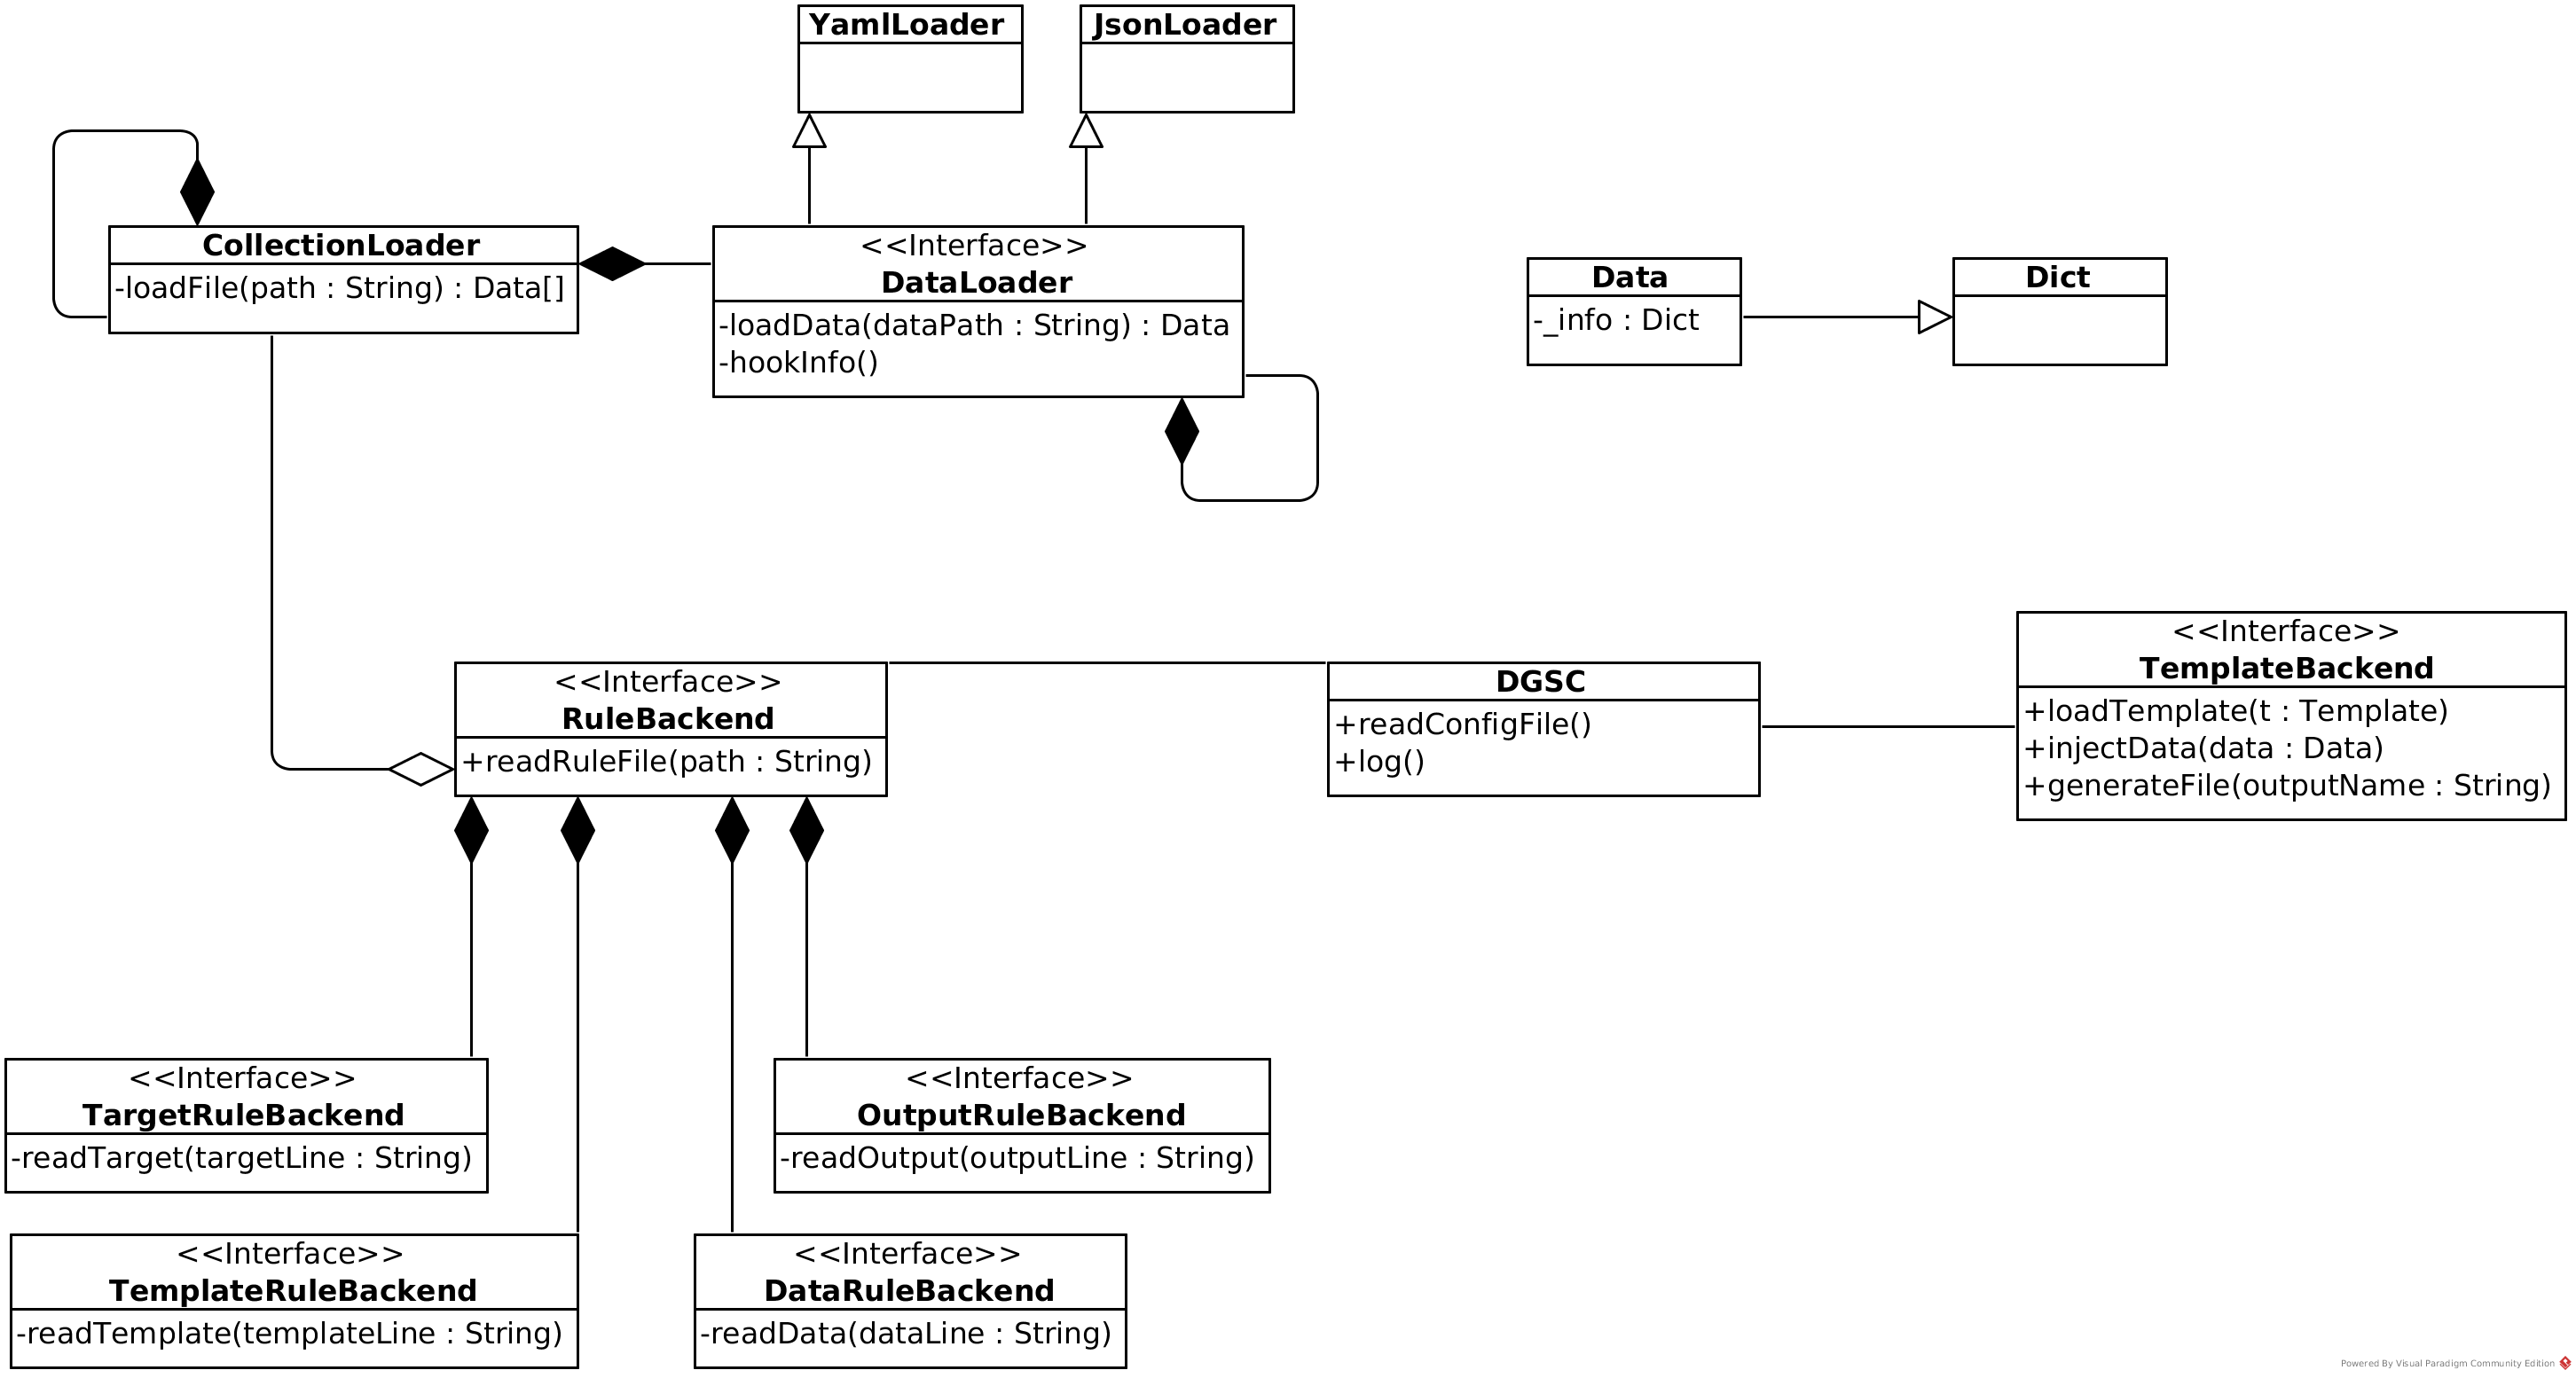
\includegraphics[width=\textwidth]{/diagrams/DGSC}
			\caption{Diagramme de classes de notre générateur de contenu statique}
			\label{fig:class_diagram}
		\end{figure} 
	
	
	\subsection{Configuration}
		Un fichier de configuration permettra à l'utilisateur de spécifier quelques options à notre générateur de contenu statique. Parmi ces options, nous retrouverons entre autres: le répertoire de travail en entrée, le répertoire de travail en sortie, une liste de classes implémentant les interfaces du générateur, l'emplacement du fichier de \textit{logs} (le cas échéant), ... Chacune de ses options aura une valeur par défaut, l'utilisateur ne devra donc spécifier que les éléments qui diffèrent de la configuration par défaut. 
\section{Conclusion}

% etc

% Si vous utilisez (conseillé) BibTeX pour votre bibliographie :
\bibliographystyle{acm}
\bibliography{memoire}% si le fichier BibTeX est memoire.bib

\end{document}
%%% Local Variables: 
%%% mode: latex
%%% TeX-master: t
%%% TeX-PDF-mode: t
%%% End: 
